\newpage
\section{Потоки сообщений EAP-PSK}

EAP-PSK включает в себя два различных типа потоков сообщений:

\begin{itemize}
\item Стандартная аутентификация:
\begin{itemize}
\item обязательна к реализации;
\item полностью описана в данном документе;
\item простейший тип потока сообщений, который, как ожидается, будет использоваться наиболее часто.
\end{itemize}
\item Расширенная аутентификация:
\begin{itemize}
\item Не обязательна к реализации;
\item Частично описана в данном документе, поскольку сильно зависит от расширений, не указанных в данном документе;
\item Тип потока сообщений, использующийся при расширении протокола EAP-PSK если от него требуются дополнительные функции.
\end{itemize}
\end{itemize}

EAP-PSK использует концепцию сессий для более легкого анализа протокла и обеспечения прозарчного интерфейса для других уровней. Сессией называется EAP-PSK взаимодействие между двумя сторонами. Каждая сессия определяется её идентификатором.

EAP сервер устанавлиает идентификатор сессии в первом EAP-PSK сообщении. Учитывая тот факт, что EAP-Request/Identity и EAP-Responce/Identity не могут предпологать, что происходило до их отправки и что данные, пересылаемые в EAP-Responce/Identity (Если такой запрос производился) может не содержать актуального NAI который Пир должен использовать с EAP-PSK мы приходим к тому, что EAP сервер, использующий метод EAP-PSK должен использовать один и тот же NAI сервера EAP для всех EAP-PSK сессий с любыми Пирами, поддерживающими EAP-PSK.

\subsection{Стандартная аутентификация EAP-PSK}

Стандартная аутентификация EAP-PSK состоит из четырех сообщений, то есть двух раундов, представленных на рисунке \ref{img:standart_aut}.

\begin{figure}[h!]
\center{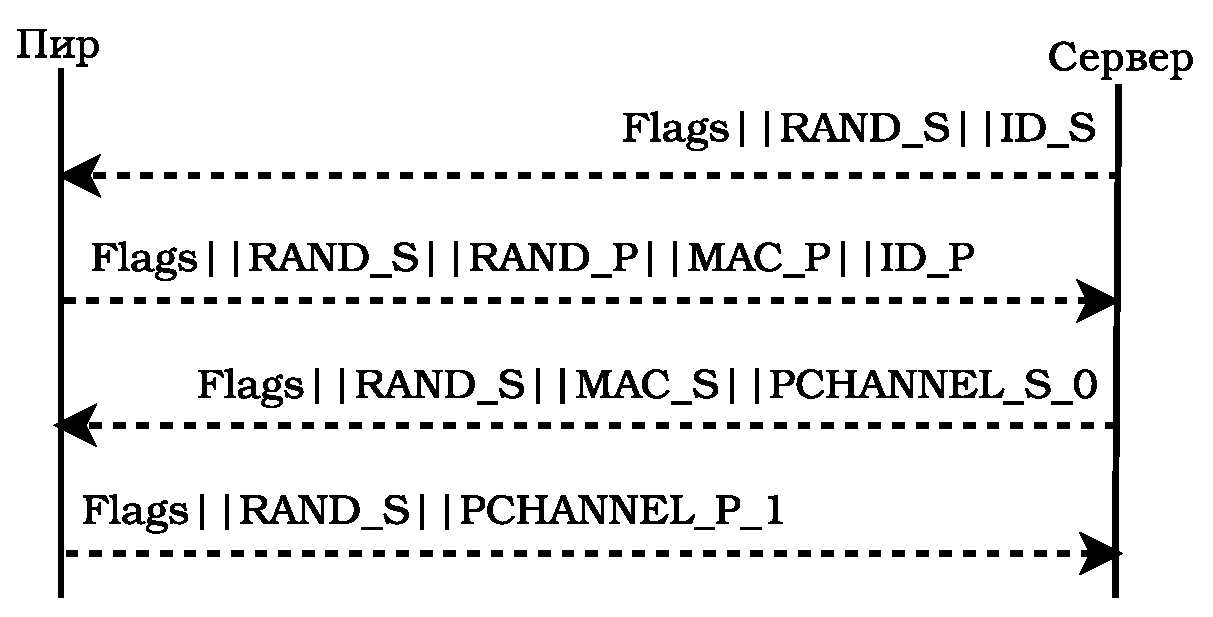
\includegraphics[width=0.9\linewidth]{./pictures/standart_aut}}
\caption{Стандартная аутентификация EAP-PSK}
\label{img:standart_aut}
\end{figure}

Первое сообщение пересылается от сервера к Пиру:

\begin{itemize}
\item Отправляется 16-байтоое случайное число RAND\_S. В разделе 3.2 обозначалось как RA;
\item Отправляется идентификатор сервера (ID\_S). В разделе 3.2 обозначалось как A.
\end{itemize}

Второе сообщение пересылается от Пира к серверу:

\begin{itemize}
\item Отправляется другое случайное число (RAND\_P). В разделе 3.2 обозначалось как RB;
\item Отправляется идентификатор Пира (ID\_P). В разделе 3.2 обозначалось как B;
\item Аутентификация на серевере, путем доказательства способности вычислить MAC (MAC\_P) при помощи функции: MAC\_P = CMAC-AES-128(AK, ID\_P||ID\_S||RAND\_S||RAND\_P).
\end{itemize}

Третье сообщение пересылается от сервера к Пиру:

\begin{itemize}
\item Аутентификация на серевере, путем доказательства способности вычислить MAC (MAC\_S) при помощи функции: MAC\_S = CMAC-AES-128(AK, ID\_S||RAND\_P);
\item Установление защищенного канала:
\begin{itemize}
\item Подтверждение получения сессионного ключа;
\item Выдача защищенной индикации результата аутентификации.
\end{itemize}
\end{itemize}

Четвертое сообщение пересылается от Пира к серверу:

\begin{itemize}
\item Подтверждение получения сессионного ключа;
\item Выдача защищенной индикации результата аутентификации.
\end{itemize}

Поля PCHANNEL\_S\_0 и PHCANNEL\_P\_1, передаваемые в третьем и четвертом сообщениях, содержится MAC, вычисленный при помощи TEK, который обеспечивает гарантию целостности сообщения. Для более детального знакомства с полями, обеспечивающими гарантию целостности сообщения необходио обратиться в раздел 3.3.

Все сообщения EAP-PSK содержат короткий заголовок, в котором есть два поля:

\begin{itemize}
\item Flags, 1-байтовое поле, которое в настоящий момент используется только для нумерации EAP-PSK сообщений;
\item RAND\_S, 16-байтовая последовательность, которая отправляется сервером в качестве идентификатора сессии.
\end{itemize}

Этот стандартный поток сообщений мог бы состоять только из трех сообщений, так же как и AKEP2, если бы не EAP-request/responce. Поскольку четвертое сообщение явлеятся обязательным, EAP-PSK использует его для установления защищенного канала.

Стандартный поток сообщений так же включает в себя выражения для Пира, при помощи которых производится его аутентификация, которые могут использоваться в дополнение к EAP-Response/Identity. Такое поведение описано в разделе 5.3 RFC3748, в котором так же сказано что рекомендуется использовать EAP-Response/Identity главным образом для маршрутизации и выбора кокнкретного метада аутентификации, следовательно, каждый EAP метод имеет свой собственный механизм идентификации и не должен полагаться на Identity Response.

Кода какая либо сторона получает сообщение EAP-PSK, она проверяет соответствие этого сообщения заданному формату, заданному в разделе 5. Если сообщение не проходит эту проверку, то сообщение игнорируется. Если проверка пройдена успешна, то производится криптографическая проверка собщения, то есть проверка MAC, которая происходит:

\begin{itemize}
\item Если получено первое сообщение EAP-PSK, то в сообщении нет MAC, так как MAC не предусмотрен в нем;
\item Если получено второе сообщение EAP-PSK, то проверяется значение MAC\_P;
\item Если получено третье сообщение EAP-PSK, то происходит проверка MAC\_S и проверка Тэга, включенного в P\_CHANNEL\_S\_0. Данная проверка должна быть зделана для того, что бы избежать генерации TEK, MSK и EMSK в случае если MAC\_S не пройдет проверку, а значит взаимная аутентификация завершится неудачей. Для проверки Тэга, включенного в P\_CHANNEL\_S\_0 используется TEK;
\item Если получено четвертое сообщение EAP-PSK, то проверяется Тэг, который включен в P\_CHANNEL\_P\_1.
\end{itemize}

Если проверка завершается неудачно, то сообщения игнорируются. Для контроля количества проигнорированных сообщений можно ввести счетчик (раздел 8.8). Если в сообщении есть зашифрованная полезная нагрузка (а именно, в PCHANNEL), то она расшифровывается. Если расшифрованная часть не проходит проверку формата, то сообщение игнорируется.

\subsection{Расширенный поток сообщений EAP-PSK}

Для сохранения простоты и возможности легкого расширения функционала EAP-PSK предоставляет механизм расширения в рамках своего защищенного канала: полезная нагрузка сообщения может содержать необязательные поля расширений (EXT).

На рисунке \ref{img:extended_aut} представлен обмен сообщениями EAP-PSK при расширенной аутентификации.

Расширенная аутентификация ДОЛЖНА поддерживаться, то есть любая реализация EAP-PSK ДОЛЖНА поддерживать отправку и получение EXT атрибутов в соответствии с правилами, описанными в разделе 6. Но, хотя поддержка EXT полей является обязательной, нет требования к обязательным типам расширений. Это означает, что если сервер запускает процедуру расширенной аутентификации EAP-PSK, а, как указано в разделе 6, такую аутентификацию может инициировать только сервер, то Пир сможет определить начало процедуры расширенной идентификации благодаря поддержки EXT полей. Если Пир не поддерживает конкретный тип расширения, используемый сервером, то Пир должен быть в состоянии завершить диалог.

Обязательная поддержка EXT полей диктуется из:

\begin{itemize}
\item гарантии корректного поведения в будущем, когда некоторые Пиры будут поддерживать некоторые расширения, а некоторые Пиры нет. Все Пиры должны быть в состоянии определить начало процедуры расширенной аутентификации и указывать поддерживают ли они то расширение, которое пытается приминить сервер;
\item гарантии того, что все реализации действительно будут поддерживать расширения.
\end{itemize}

В настоящее время ни одно расширение не было определено.

В большинстве случаев одно расширение может быть использовано в рамках одного EAP-PSK обмена: не может запускаться последовательность из нескольких расширений или параллельное использование несколькиз расширений. Тем не менее, расширения могут использвать различное число раундов обмена для завершения.

Только сервер может запустить расширение и, если он делает это, то должен инициировать его в первом сообщении, отправленном внутри установленного защищенного канала.

\begin{figure}[h!]
\center{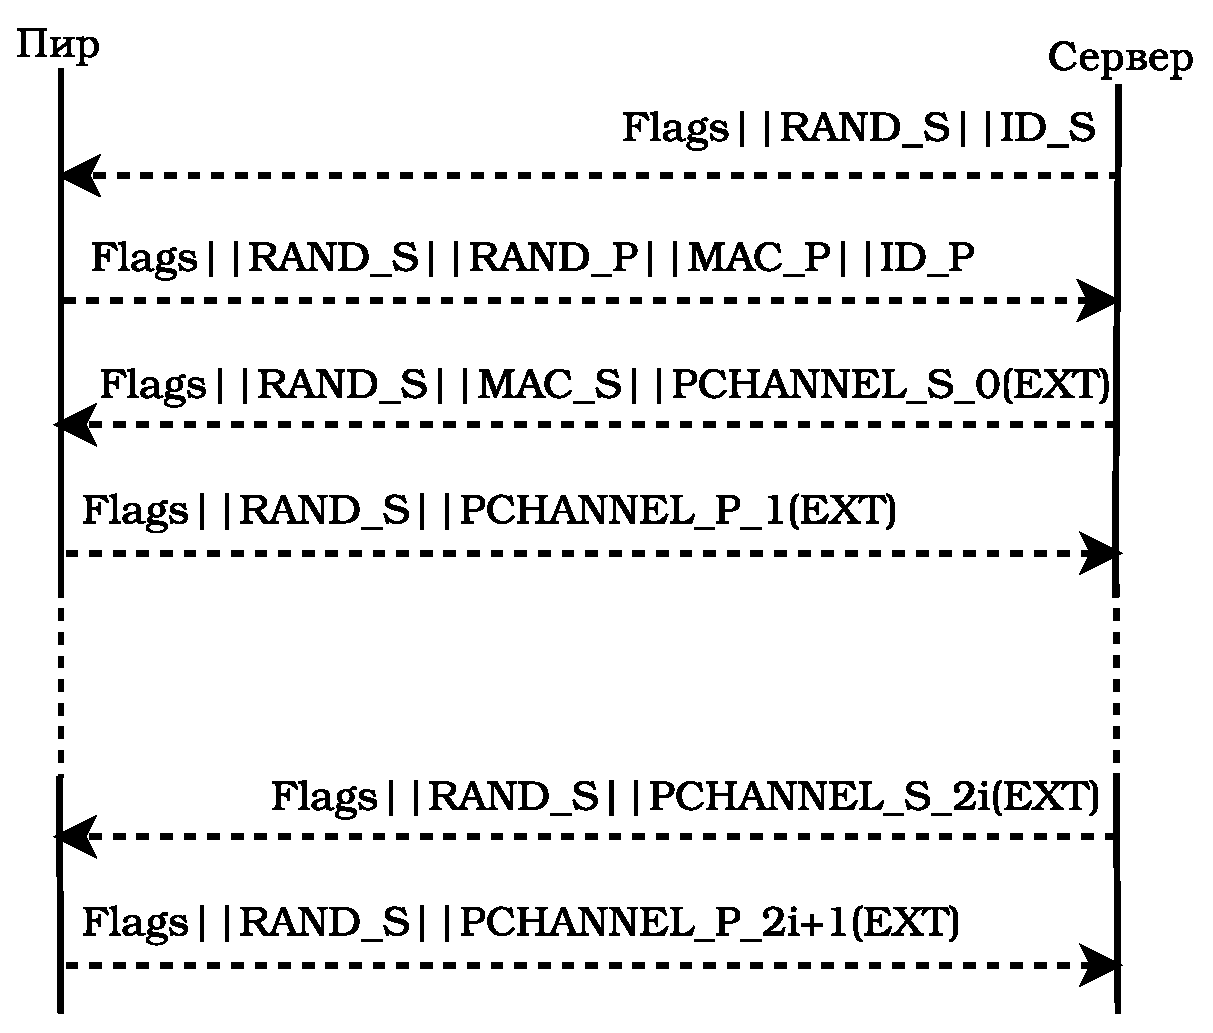
\includegraphics[width=0.9\linewidth]{./pictures/extended_aut}}
\caption{Расширенная аутентификация EAP-PSK}
\label{img:extended_aut}
\end{figure}
